%%=============================================================================
%% Methodologie
%%=============================================================================

\chapter{Methodologie}
\label{ch:methodologie}

%% TODO: Hoe ben je te werk gegaan? Verdeel je onderzoek in grote fasen, en
%% licht in elke fase toe welke stappen je gevolgd hebt. Verantwoord waarom je
%% op deze manier te werk gegaan bent. Je moet kunnen aantonen dat je de best
%% mogelijke manier toegepast hebt om een antwoord te vinden op de
%% onderzoeksvraag.

\section{Wat zijn de redenen van een omschakeling?}
\label{sec:methodologie-redenen-omschakeling}

TO DO
- slechte monitoring
- slecht geautomatiseert 
- geen multi environment
- expert vertrokken
- gui veel werk en complex
- oorspronkelijk geen modules, refactor, in feite nu weer refactor
- updates zorgen voor compatiblieteistproblemen (denk ik)
- puppet client niet ouder dan puppet master maar omgekeerd denkik wel (op te zoeken)

\section{Technische werking van Ansible en Puppet?}
\label{sec:methodologie-technische-verschillen}

\subsection{Overzicht van Puppet en Ansible}

\begin{minipage}{15cm}
\begin{tabular}{ r |c c }
& \textbf{Ansible} & \textbf{Puppet} \\
  \hline	  		
Programmeerparadigma\footnote{synoniemen zijn ook programmeerstijl of programmeermodel, voorbeelden zijn object-geori\"onteerd, procedureel, imperatief..., \autocite{journalofinformation} }  & declaratief & declaratief  \\
   \hline
 Programmeertaal & YAML & eigen DSL  \\
     \hline
   Communicatieprotocol & SSH & HTTPS \\
   \hline
   open poorten\footnote{Dit zijn de minimale vereisten van open poorten. Voor sommige features dienen meer poorten open te staan. Bijvoorbeeld 443 voor Ansible Tower of 8140 op elke Puppetclient voor de puppet kick functionaliteit \autocite{puppetkick} }  & 22/tcp (client) & 8140/tcp (master)\\
  \end{tabular}
  \end{minipage}   



 \autocite{languagePuppet}\autocite{masterproef} \autocite{ansibledoc}

\subsection{Werking van Puppet}

Tussen de master en de client bestaat er een vertrouwensrelatie die onderhouden wordt door certificaten. Het is de Puppetmaster die verantwoordelijk is voor het verlenen van deze certificaten. Pas als deze in orde zijn kan Puppet  aan de configuraties van de clients beginnen. De code die je schrijft wordt een manifest genoemd. Wanneer een Puppetagent wil controleren of hij nog up-to-date is, zal hij een catalogus aanvragen bij de Puppetmaster. Een dergelijke catalogus is in feite een manifest dat de Puppetmaster compileert. Deze catalogus is bovendien uniek voor elke Puppetagent. Dit komt omdat er bij het compileren van het manifest naar de catalogus rekening gehouden wordt met diverse parameters zoals de functie van de server of de distributie van het besturingssysteem dat op die server draait \autocite{Puppetlanguagecatalog}. Eens de Puppetagent zijn persoonlijke catalogus ontvangen heeft, zal deze voor zichzelf controleren of er verschillen zijn tussen zijn huidige configuratie en de staat die beschreven staat in de catalogus. Indien er afwijkingen zijn, worden deze ook automatisch opgelost \autocite{Puppetdoc}.

\begin{figure}  \begin{center}
  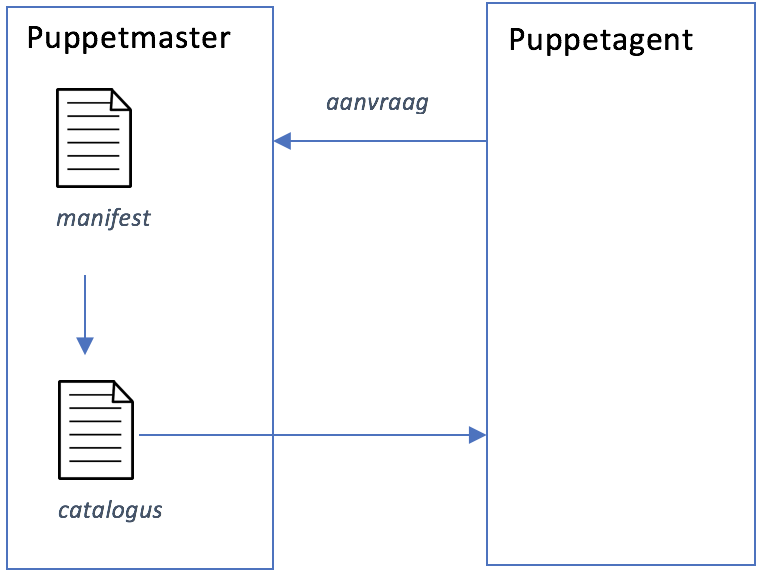
\includegraphics[width=250px]{img/aanvraagCatalogus.png}
 \end{center}\caption{aanvraag van een catalogus bij de Puppetmaster door een Puppetclient. De Puppetagent is een deamon (stukje software) die op de Puppetclient draait.}  
  \label{fig:aanvraagCatalogus}
\end{figure}


\subsection{Werking van Ansible}

Ansible maakt geen gebruik van agenten. Dit betekent dat de Ansibleserver enkel de naam en het wachtwoord dient te kennen van de servers die hij moet configureren. Het authenticeren kan op verschillende manieren. Er wordt aangeraden om gebruik te maken van een SSH-key, wat het eenvoudigst is, maar ook andere middelen zoals met een eenvoudig wachtwoord of het Kerberos-protocol worden ondersteund. De gewenste configuraties worden geschreven in playbooks met bijhorende modules. Eens een verbinding tot stand is gebracht wordt dit playbook met zijn modules verstuurd naar de te configureren server. Deze worden vervolgens op de Ansible clients uitgevoerd  en weer verwijderd. Ook Ansible bezit de functionaliteit om na te gaan of de huidige configuratie in lijn is met de ontvangen modules. Om servers te configureren met Ansible bestaan er bovendien twee manieren. Ansible playbooks kunnen in principe verstuurd worden naar de servers vanaf elke computer. Voor een grotere hoeveelheid servers is dit echter niet aangeraden en bestaat er de commerci"ele versie waarbij de playbooks worden verstuurd vanaf een centraal punt. Dit centraal punt is voorzien van Ansible Tower die een inventaris heeft van alle servers en playbooks die onder zijn verantwoordelijkheid vallen \autocite{ansibledoc}.


\subsection{Performantie}

Het is interessant om te weten wat de verhoudingen zijn tussen de deploy-tijd tussen Ansible en Puppet. Om dit op zo een betrouwbare mannier te kunnen verwezelijken zijn de configuraties van Ansible en Puppet zo analoog mogelijk gehouden en worden dus dezelfde services ge\"installeerd en geconfigureerd. Vervolgens wordt elke configuratie 30 keer uitgevoerd. De tijd kan worden onderverdeeld in twee delen.\newline
Het eerste deel van de tijd zal de connectietijd genoemd worden. Dit is de tijd die het kost totdat er effectief overgegaan kan worden tot configureren. Hieronder zitten zaken zoals het opstellen van een verbinding, het verzamelen van nodige gegevens en het versturen van een gepersonaliseerde configuratie. Bij Ansible kon deze tijd gewoon berekend\footnote{connectietijd = totaal verstreken tijd -  \unexpanded{$ \sum  $} (tijd playbooks)} worden op basis van de resultaten. Bij Puppet is dit echter niet mogelijk en bijgevolg zijn deze resultaten met de hand gemeten.\newline
 De tweede tijd is de tijd die nodig is om de configuratie effectief uit te voeren. Beide waarden zijn gebasseerd op de feedback van de corresponderende CMT.

\textbf{Tijd tot het bekomen van een verbinding (connectietijd)} (in seconden) \newline
\begin{tabular}{| r |c |c |c |c |c |c |c |c |c |c |c |c |c |c |c |c |c |c |c |c |c |c |c |c |c |c |c |c |c |c |c |c |c |c |}
  \hline	  		
Puppet & 9 & 6 & 6 & 11 & 6 & 7 & 8 & 6 & 9 & 9 & 7 & 7 & 8 & 6 & 6   \\ 
\hline
& 9 & 10 & 8 & 8 & 7 & 10 & 8 & 6 & 5 & 5 & 5 & 5 & 7 & 6 & 15\\
   \hline    \hline
  Ansible & 9 & 5 & 5 & 7 & 4 & 5 & 6 & 5 & 4 & 11 & 6 & 4 & 8 & 10 & 7 \\ 
\hline
   & 5 & 6 & 4 & 9 & 5 & 11 & 13 & 13 & 8 & 12 & 8 &	7 & 7 & 8  & 10 \\
  \hline  
\end{tabular}


\textbf{Tijd tot het bekomen van een consistente staat (deploytijd)} (in seconden)

\begin{tabular}{| r |c |c |c |c |c |c |c |c |c |c |c |c |c |c |c |c |c |c |c |c | c c |}
  \hline			
  
Puppet & 51,35 & 43,56 & 46,78 & 55,18 & 40,59 & 47,01 & 35,99 & 35,07 & 43,29 & 42,28  \\ \hline
           & 42,20 & 96,83 & 32,33 & 49,99 & 40,32 & 55,62 & 52,82 & 42,72 & 44,21 & 43,13 \\ \hline
            & 47,43 & 56,98	& 59,97 & 61,28 & 53,98	& 56,56 & 53,57 & 49,01 & 50,21 & 51,30 \\ \hline
              \hline 
   
  Ansible & 67 & 60 & 51 & 59 & 51 & 51 & 59 & 57 & 45 & 90 \\ \hline
                & 52  & 53 & 54 & 52 & 62 & 68 & 51 & 59 & 53 & 45  \\ \hline
                & 96 & 73 & 61 & 62	& 59 & 64	& 65 & 64 & 76 & 61  \\ \hline
                
  \hline  
\end{tabular}


\subsubsection{Deploytijd}
\begin{figure}
  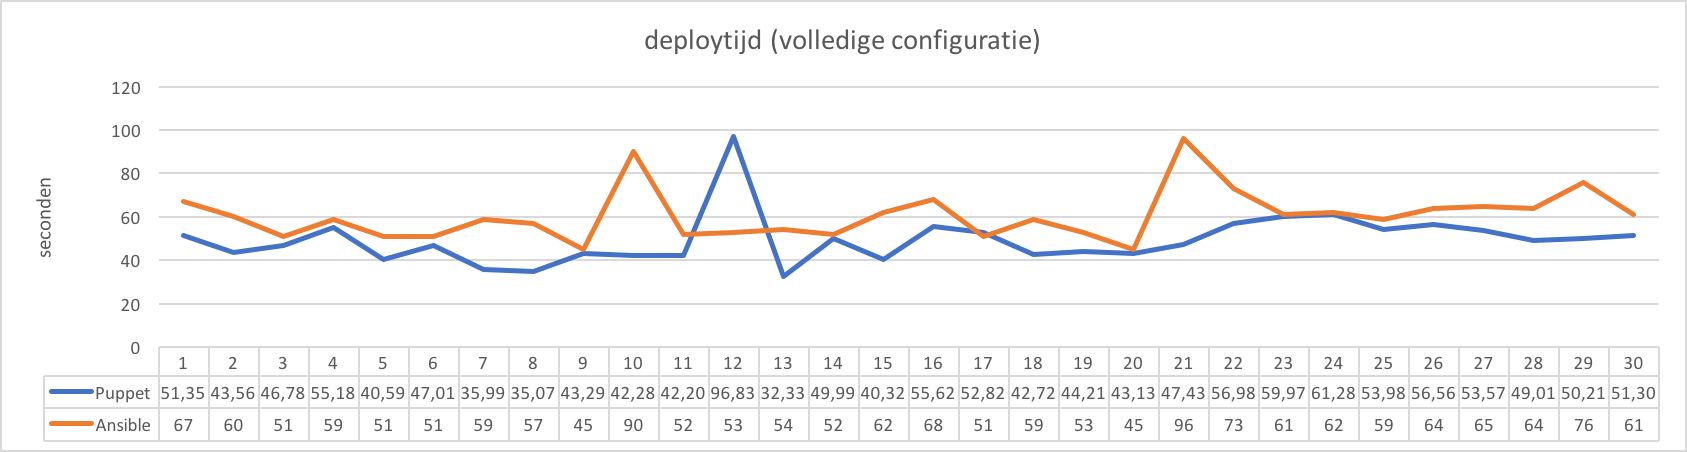
\includegraphics[width=\linewidth]{img/deploytime_fullconfig.png} 
  \caption{Tijd tot het bekomen van een consistente staat, vertrekende van een 'lege' server.}  
  \label{fig:deploytime_fullconfig}
\end{figure}

Aangezien grafiek \ref{fig:deploytime_fullconfig} geen duidelijk verschil toont tussen beide CMT's zal met behulp van de Z-toets aangetoond worden of er al dan niet een statistisch verschil is.

\underline{Hypothese}
\begin{align*}
H_0:  \mu_p = \mu_a \\
H_a: \mu_p\neq \mu_a 
\end{align*}


\underline{Significantieniveau en waarden} \newline

 $\alpha$ = 0.05 => -1.96 en +1.96 \newline

		\begin{tabular}{ r |c |c }
			& Puppet & Ansible\\\hline
			\unexpanded{$ \bar x  $} &  60.7 & 49.4\\ \hline
			$\sigma$ & 11.5 & 11.6\\ \hline
			n &  30 &  30

\end{tabular}


\underline{Toetsingsgrootheiden}
\begin{equation} \label{eq1}
\begin{split}
Z &= \tfrac{\bar x_p - \bar x_a}{\sqrt{\tfrac{\sigma_p^2}{n_p}+\tfrac{\sigma_a^2}{n_a}}}\\
& = \tfrac{49,4 - 60,7}{\sqrt{\tfrac{11,6^2}{30}+\tfrac{11,5^2}{30}}} \\
& = -3,789
\end{split}
\end{equation}



\underline{Conclusie} \newline
Z valt buiten het kritisch gebied waardoor de nulhypotese verworpen kan worden. Bijgevolg wordt aangenomen dat beide gemiddelde niet tot dezelfde verzameling behoren. Er kan dus worden geconcludeerd dat wanneer er wordt vertrokken van een lege server, Ansible er gemiddeld langer over doet dan Puppet. Dit is in dit geval een verschil van 11,3 seconden. \newline

De verschillen worden echter nog groter wanneer de test gedaan wordt met een gedeeltelijke configuratie. Hiermee wordt bedoelt dat er is vertrokken van servers die reeds geconfigureerd zijn en slechts enkele aanpassingen moeten doorgevoerd worden. Deze aanpassingen zijn een service starten en de inhoud van de webpagina veranderen. De resultaten lopen niet door elkaar waardoor een Z-toets niet echt nodig is. Ansible deed gemiddeld 19,10 seconden voor de deploy met een vrij grote variatie van 33,40 seconden. Puppet haalde maar een vrij consistente 3,10 seconden met een variatie van 0,35. \newline

In laatste instantie is er gekeken naar de tijd die het zou kosten totdat de CMT vaststelt dat de server reeds volledig is geconfigureerd en dat geen aanpassingen nodig zijn. Hierbij resulteert Ansible op een gemiddelde van 18 seconden met opnieuw een vrij grote variatie van 18,25 seconden. Ook hier doet puppet het opnieuw beter waarbij Puppet er minder dan een seconde nodig heeft om vast te stellen dan dat geen aanpassingen nodig zijn. Uiteraard zijn al deze waarden afhankelijk van de configuratie maar ze geven wel een duidelijke indicatie van de verschillen tussen beide CMT's.

\textbf{Opmerking:} De connectietijd is niet meegerekend in deze metingen. Het omvat hier uitsluitend de deploy tijd.
\subsubsection{Connectietijd}
Ook hier lopen de resultaten door elkaar zoals te zien is op grafiek \ref{fig:connectiontime}, bovendien liggen de gemiddelden hier veel dichter bij elkaar. Om vast te stellen of er een significant verschil zal er opnieuw gebruik gemaakt worden van de Z toets.
\begin{figure}
  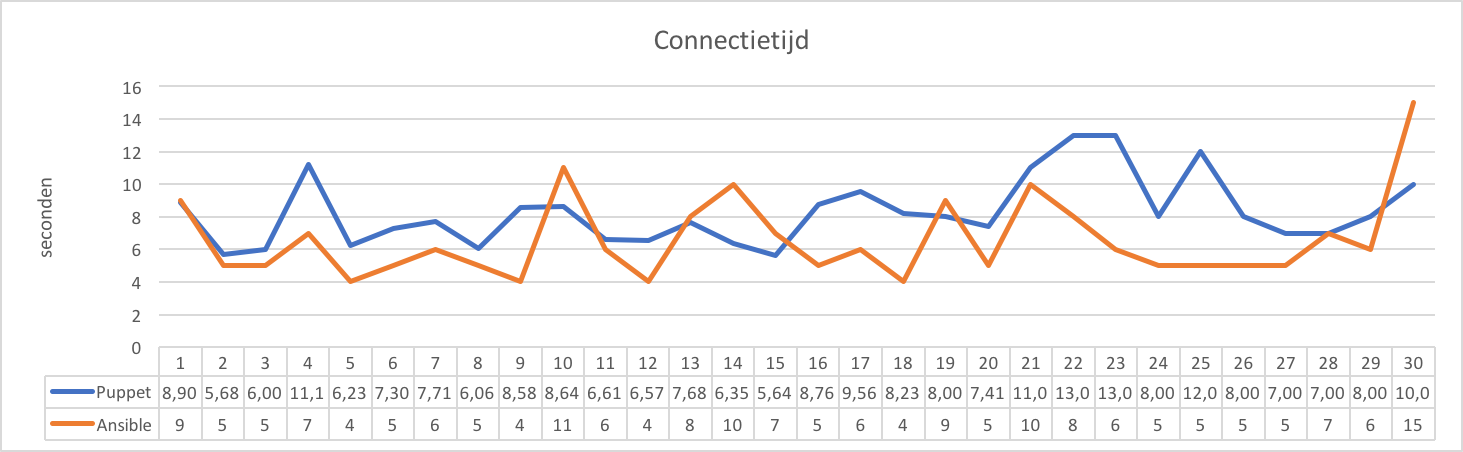
\includegraphics[width=\linewidth]{img/connectiontime.png} 
  \caption{Tijd tot het initialiseren van de deploy}  
  \label{fig:connectiontime}
\end{figure}



\underline{Hypothese}
\begin{align*}
H_0:  \mu_p = \mu_a \\
H_a: \mu_p\neq \mu_a 
\end{align*}
\underline{Significantieniveau en waarden} \newline

 $\alpha$ = 0.05 => -1.96 en +1.96 \newline

		\begin{tabular}{ r |c |c }
			& Puppet & Ansible\\\hline
			\unexpanded{$ \bar x  $} &  6,27 & 6,57\\ \hline
			$\sigma$ & 4,10 & 6,11\\ \hline
			n &  30 &  30

\end{tabular}


\underline{Toetsingsgrootheiden}
\begin{equation} \label{eq1}
\begin{split}
Z &= \tfrac{\bar x_p - \bar x_a}{\sqrt{\tfrac{\sigma_p^2}{n_p}+\tfrac{\sigma_a^2}{n_a}}}\\
& = \tfrac{ 6,27 - 6,57}{\sqrt{\tfrac{ 4,10 ^2}{30}+\tfrac{ 6,11^2}{30}}} \\
& = 1,27
\end{split}
\end{equation}
\underline{Conclusie}\newline
Z ligt in het aanvaardingsgebied waardoor we de nulhypothese, die stelt dat beide gemiddelden gelijk zijn, kunnen aanvaarden. Er is bijgevolg geen statistisch verschil tussen beide waarden.

%%---------------------------------------------------- einde performantie
\subsection{Belasting van het netwerk}

Ansible en Puppet hebben een groot verschil in de manier van communiceren en dit weerspiegeld zicht in het gedrag van de CMT. Op afbeelding \ref{fig:netwerkverbruikpernode} bevinden zich links alle Ansible clients, te herkennen aan hun naam die begint met een A. Rechts staan alle puppet clients, te herkennen aan de PP. De grafieken weerspiegelen uitsluitend het dataverkeer tussen de server (Ansible Tower of Puppetmaster) en de desbetreffende client. Andere data, zoals bijvoorbeeld het downloaden van services of uploaden van logbestanden naar de monitoringstool zijn hierin \underline{niet} opgenomen. Dit wordt verwezenlijkt door gebruik te maken van verschillende netwerkkaarten. Wanneer er geen deploy gebeurt is de kilobyte/ minuut op deze netwerkkaart gelijk aan nul, een bewijs dat hier geen andere data dan deze van de CMT over wordt verstuurd.  \newline

De mannier van communicatie is te herkennen in de grafieken. Zo onderhoud Ansible de communicatie met de client gedurende de deploy. Hiermee wordt bedoelt dat Ansible op de hoogte is van de laatste stand van zaken op de client. Wanneer een bepaalde taak voltooid is wordt Ansibel Tower hier onmiddelijk van op de hoogte gebracht. Zoals te zien is op de grafiek \ref{fig:deploytypes} is er geregeld communicatie tussen beide servers. Welliswaar is er enkel communicatie wanneer iets voltooid is, er is dus geen onnodige communicatie. Zo is ook te zien hoe op t6 de communicatie nul is. Ansible had voor die periode niets te melden\footnote{Hier betreft het de service MariaDB die werd ge\"installeerd}. \newline
 Deze mannier van werken is handig tijdens het schrijven van nieuwe Ansible rollen. Je krijgt namelijk live feedback tijdens het uittesten. Een nadeel hieraan is dat het netwerk geen rust krijgt. Bovendien word deze functionaliteit van 'live feedback' in productie niet vaak gebruikt. In realiteit lopen deze jobs tijdens de nacht en is het voldoende om de dag erop een algemeen overzicht te krijgen.\newline

Bij puppet is dit anders. Hierbij is er enkel communicatie tussen de server en de client op het begin en het einde van de deploy. Opmerkelijk hierbij is dat er twee types te herkennen zijn. Op figuur \ref{fig:deploytypes} zijn deze Puppet type A en B genoemd. Bij Puppet type A is te zien hoe de deploy bestaat uit twee reeksen terwijl dit bij type B uit drie reeksen bestaat. De oorzaak van deze derde reeks is niet gekend. Het opnieuw versturen van de tweede reeks was tijdelijk een piste maar dit is vermoedelijk niet het geval. Moest er een tcp-pakketje verloren gegaan zijn zou uitsluitend dat pakketje opnieuw verstuurd worden en niet de hele reeks. Verder heeft de poging om de inhoud van de pakketjes te lezen tot niet veel geleid. De verbinding is namelijk ge\"encrypteerd door het HTTPS-protocol met als gevolg dat tools zoals Wireshark of tcpdump geen oplossing konden bieden over de inhoud hiervan.\newline
Een nadeel aan het feit dat er enkel in het begin en het einde communicatie is, is dat er op de master geen live feedback voor testen gevolgd kan worden. Dit kan echter wel opgelost worden door in te loggen op de client en hier de live feedback volgen met het commando 'puppet agent -t'. Het wordt wel nog steeds pas op het einde van de deploy terug naar de master gestuurd?
 \newline


Vervolgens is er ook gekeken naar de totale netwerkbelasting. Hiervoor is er per client een cumulatie genomen van de kilobytes/minuut gedurende de gehele deploy. Deze waarden zijn terug te vinden in grafiek \ref{fig:netwerkverbruik}. Hier heeft Ansible een gemiddelde van 5802,29 kilobytes/deploy. Puppet heeft bij deploy's van type A (bestaande uit twee reeksen) een gemiddelde van  9392,5 kilobytes/deploy en bij type B (bestaande uit drie reeksen) 13742,35 kilobytes/deploy. Gezamenlijk heeft Puppet een gemiddelde van 11777,90 kilobytes/deploy. 


\begin{figure}
  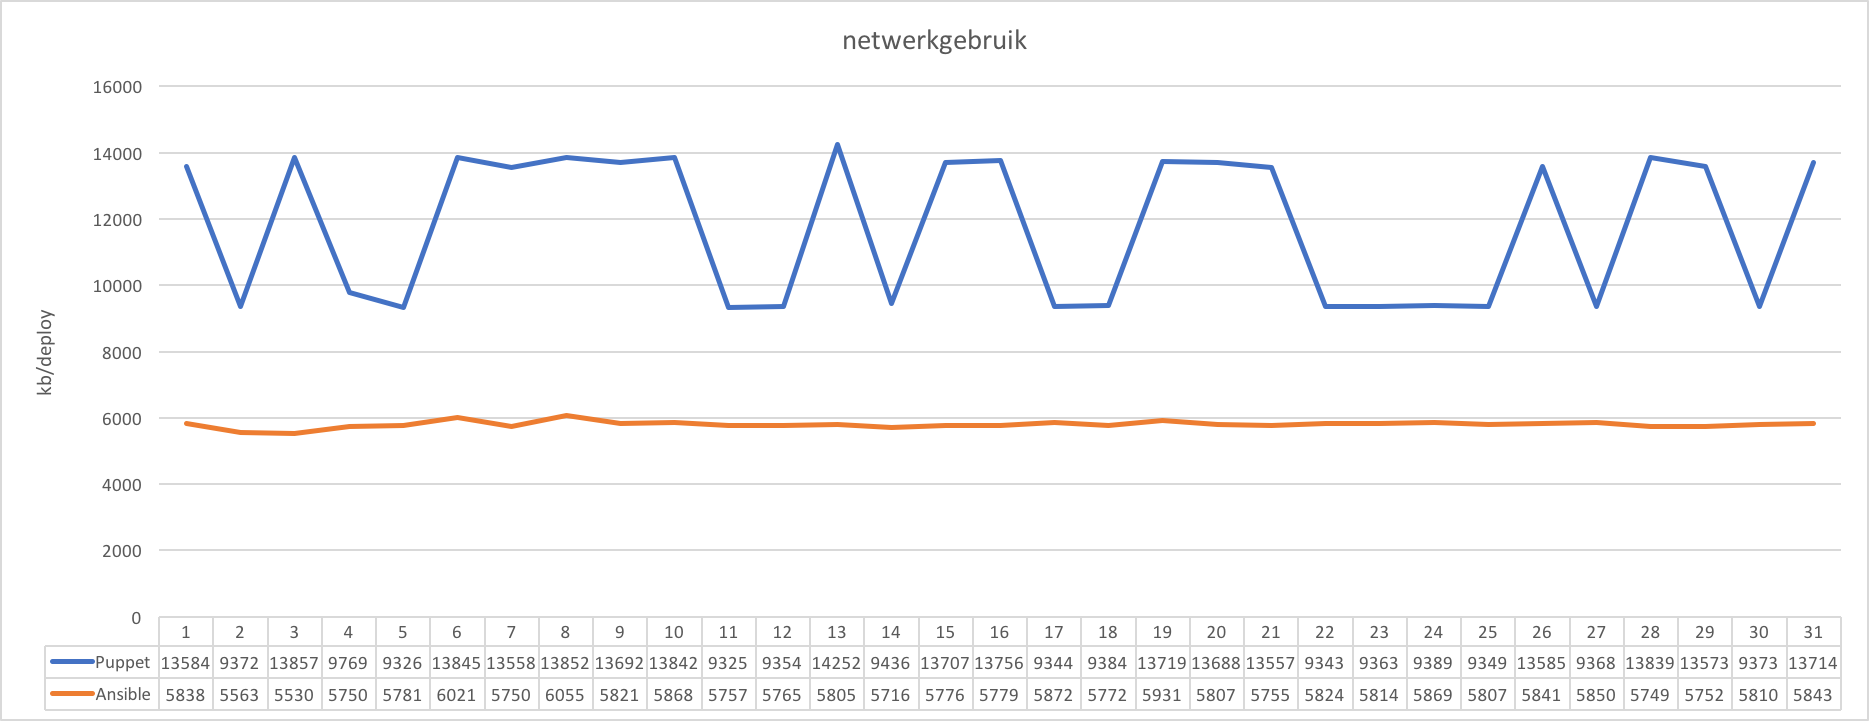
\includegraphics[width=\linewidth]{img/netwerkverbruik.png}
 \caption{Totaal verbruikte netwerkcapaciteit per client gedurende het deployen. Dit bevat enkel communicatie tussen master en client.}  
  \label{fig:netwerkverbruik}
\end{figure}


\begin{figure}
  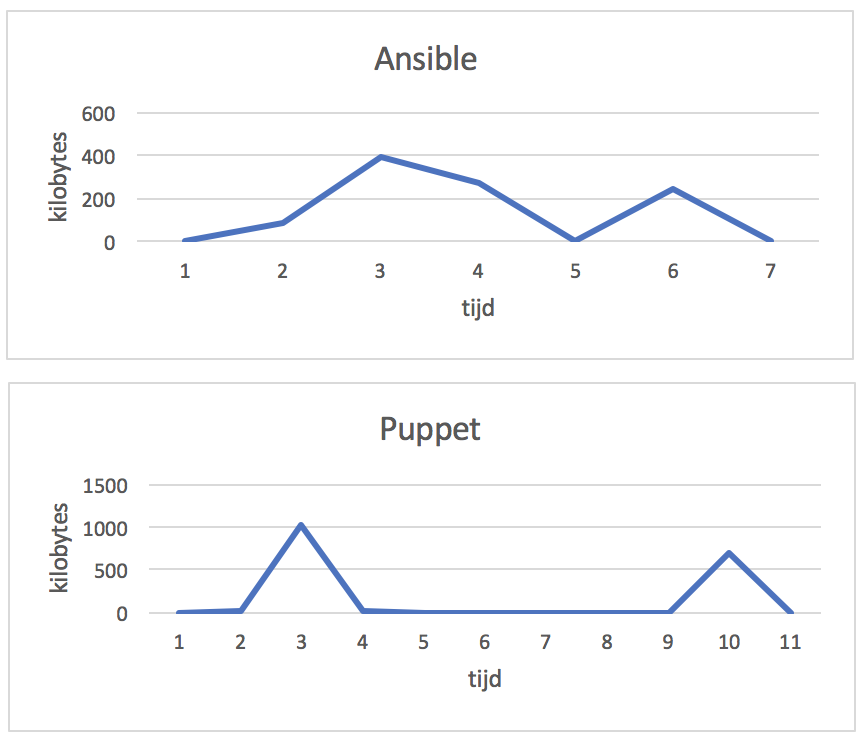
\includegraphics[width=\linewidth]{img/deploytypes.png}
 \caption{Drie types van communicatie. Aantal kilobytes per tijdseenheid op een netwerkkaart die uitsluitend bedoelt voor communicatie met Ansible Tower / Puppetmaster. }  
  \label{fig:deploytypes}
\end{figure}

\subsection{Gebruik van het geheugen}

Op grafiek \ref{fig:geheugengebruik} is per tijdseenheid het gemiddelde gebruikte ramgeheugen weergegeven. Hierop is te zien hoe Puppet opvallend meer geheugen gebruikt. Niet alleen tijdens een deploy maar ook ervoor en erna. Zelfs wanneer een Ansible client en een Puppet client juist opgezet worden met behulp van de Vagrantfile is er al een verschil in het gebruikte geheugen. Gezien het feit dat er al een verschil waar te nemen is in deze vroege levensfase van de server en het enige verschil in configuratie op dit moment de Puppetagent is werd vermoed dat het verschil hier aan te wijten is. Dit vermoeden werd gestaafd toen de Puppetagent tijdelijk uitgezet werd. Het ramgeheugen daalde onmiddelijk naar gelijkwaardige waarden als deze van de Ansibleclient. Zonder configuratie gebruiken Puppetclients gemiddeld 58\% geheugen van de 500MB ram. Bij Ansible is dit 47\%. Dit betekend dat met een verschil van 11\% er bij 500 MB, 55MB meer RAM-geheugen gebruikt wordt bij Puppet.


\begin{figure}
  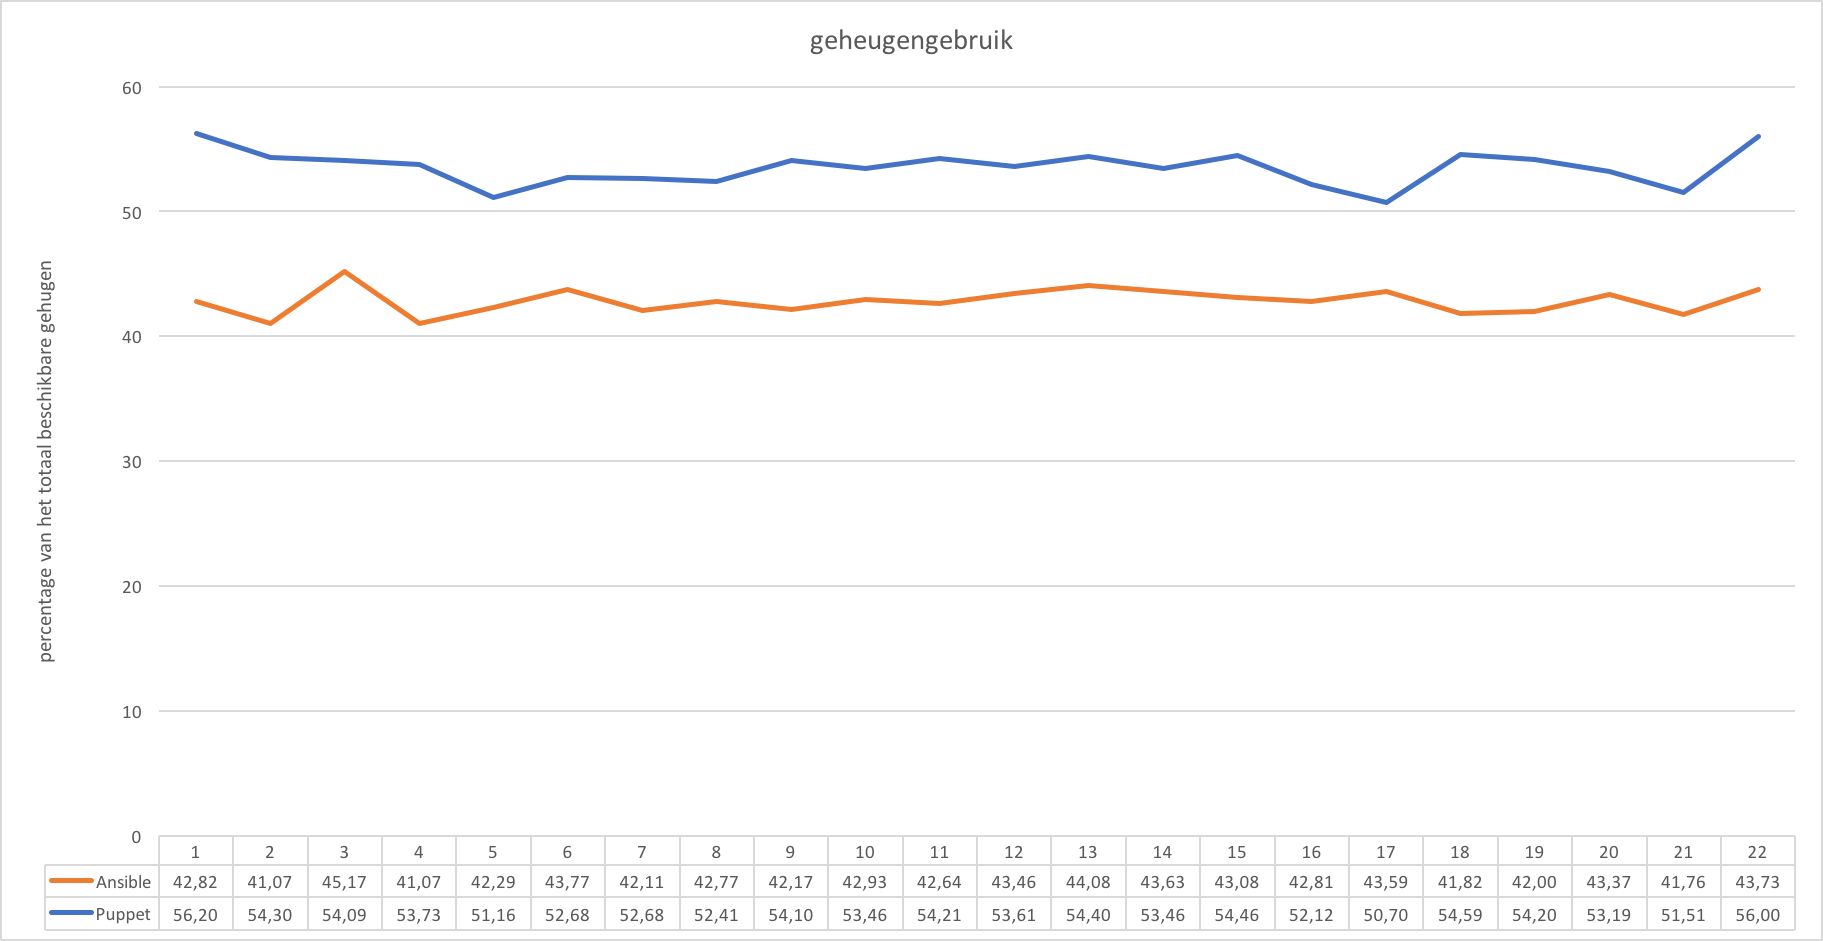
\includegraphics[width=\linewidth]{img/geheugengebruik}
 \caption{Verbruikt percentage van het RAM geheugen. Gemeten bij servers met elk 500 MB. }  
  \label{fig:geheugengebruik}
\end{figure}




\section{Wat is het verloop van een dergelijke transitperiode?}
\label{sec:methodologie-verloop-transit}









